\chapter{数据库原型的设计与实现}
本章的将基于前序章节中关于分布式数据库的建模和分析，以及经\TLAPlus 验证过的支持混合隔离级别的分布式数据库操作语义，设计并实现一个数据库原型系统，用于验证该操作语义相较于只支持单一隔离级别的操作语义在性能上的优势。

\section{需求分析}
本文中的数据库原型系统旨在实现一个分布式数据库原型，用于验证支持混合隔离级别的操作语义相较于单一隔离级别操作语义在性能上的优势。为了满足这一目标，需要对设计目标进行需求分析，明确系统的功能需求和非功能需求。

\subsection{功能需求}
功能需求定义了系统必须完成的具体任务和行为。基于验证混合隔离级别性能优势的目标，系统的主要功能需求如下：

\begin{enumerate}
    \item \textbf{基本数据操作}：本原型系统作为一个键值（Key-Value）数据库，需支持基本的读（Get）、写（Put）、增（Insert）、删（Delete）四种数据操作。数据模型以键值对（Key-Value）形式存储，不支持复杂的嵌套文档结构。
    \item \textbf{分布式集群管理}：
          \begin{itemize}
              \item \textbf{分片（Sharding）}：支持将数据水平切分并分布在多个分片节点上。
              \item \textbf{路由（Routing）}：客户端通过路由节点访问数据，路由节点根据分片键将请求转发至正确的分片。
          \end{itemize}
    \item \textbf{事务管理}：
          \begin{itemize}
              \item \textbf{事务生命周期}：支持事务的开启（Start）、提交（Commit）和中止（Abort）。
              \item \textbf{跨分片事务}：支持涉及多个分片的分布式事务，保证原子性。
          \end{itemize}
    \item \textbf{混合隔离级别支持}：这是本系统的核心需求。系统允许客户端在开启事务时指定该事务的隔离级别。系统应至少支持以下几种隔离级别的混合运行：
          \begin{itemize}
              \item \textbf{并行提交（Parallel Committed, PC）}
              \item \textbf{并行快照隔离（Parallel Snapshot Isolation, PSI）}
              \item \textbf{快照隔离（Snapshot Isolation, SI）}
              \item \textbf{可串行化（Serializable, SER）}
          \end{itemize}
          系统需要确保在上述隔离级别混合运行时，不仅能保证各自隔离级别的语义，还能保证数据的一致性和正确性。
\end{enumerate}

\subsection{非功能需求}
非功能需求涉及系统的性能、可靠性等方面：
\begin{enumerate}
    \item \textbf{高性能}：由于采用了全内存存储，系统应具有较低的读写延迟和较高的吞吐量。
    \item \textbf{可扩展性}：系统应支持水平扩展，通过增加分片节点来线性提升存储和处理能力。
    \item \textbf{可观测性}：为了验证性能优势，系统必须提供详细的性能监控指标（如延迟、吞吐量、冲突率等），以便进行后续的实验对比。
\end{enumerate}

\subsection{用例分析}
系统主要涉及两类角色：客户端用户（Client）和系统管理员（Admin）。
\begin{itemize}
    \item \textbf{客户端用户}：主要进行数据的读写操作和事务处理。他们可以发起普通读写请求，也可以开启特定隔离级别的事务进行一系列操作。
    \item \textbf{系统管理员}：负责集群的配置，如添加分片、配置路由规则等。
\end{itemize}

用例图~\ref{fig:usercase}展示了系统的核心用例。其中，“执行混合隔离级别事务”是本系统的特色用例，用户在开启事务时可以选择所需的隔离级别（RC, SI, SER）。

\begin{figure}[htbp]
    \centering
    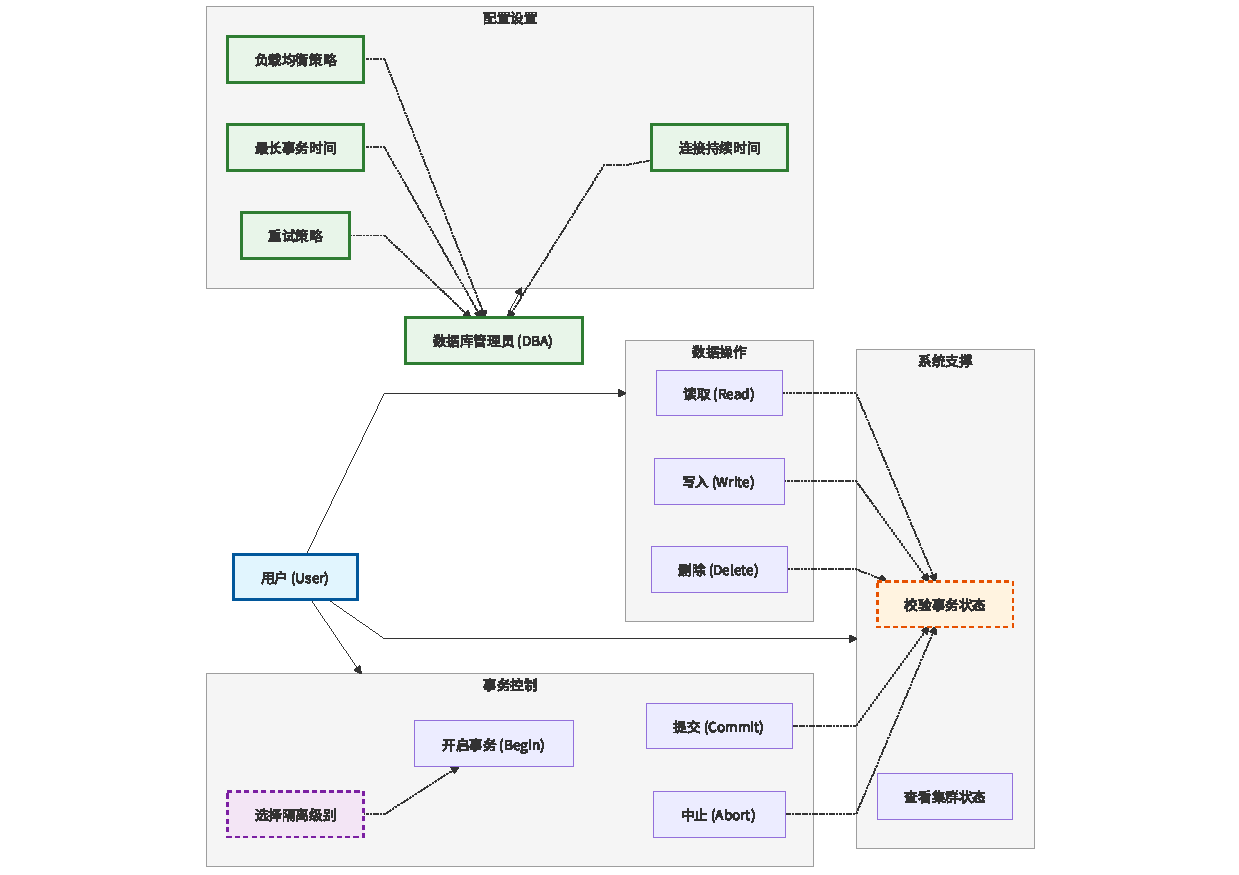
\includegraphics[width=1.0\textwidth]{figures/usercase.pdf}
    \caption{系统用例图}
    \label{fig:usercase}
\end{figure}

\section{系统设计}
基于上述需求分析，本节将对数据库原型系统进行总体架构设计和模块设计。

\subsection{总体架构设计}
本系统采用经典的 Shared-nothing 分布式架构，参考 MongoDB 的集群模型，主要由三类组件构成：路由节点（Router）、配置节点（Config Server）和分片节点（Shard Server）。

\begin{figure}[htbp]
    \centering
    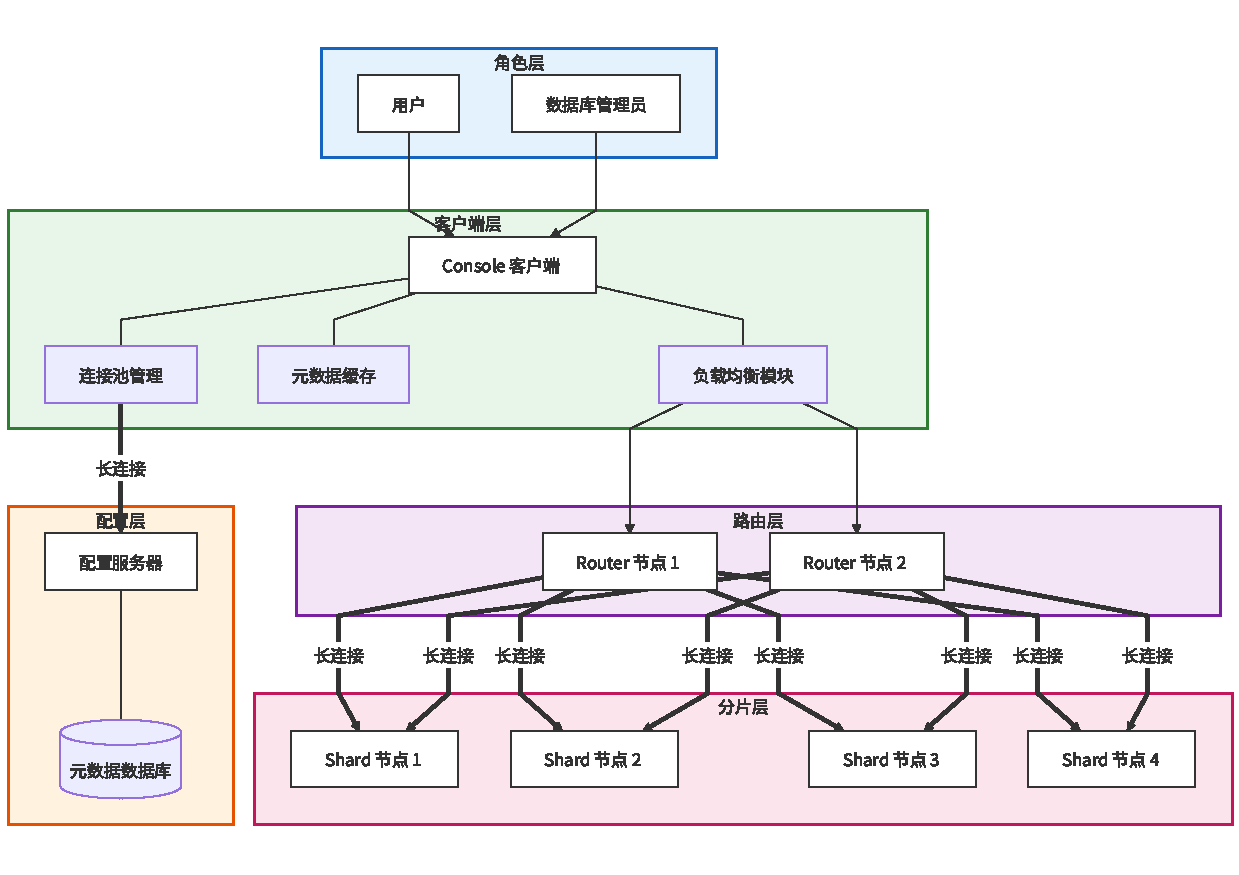
\includegraphics[width=0.8\textwidth]{figures/architecture.pdf}
    \caption{系统总体架构图}
    \label{fig:architecture}
\end{figure}

各组件职责如下：
\begin{itemize}
    \item \textbf{路由节点（Router）}：
          作为集群的统一入口，对外提供以 MySQL 或自定义协议的接口。
          路由节点不存储实际数据，只缓存元数据（Metadata）。
          它负责解析客户端请求，根据分片键（Shard Key）和路由表（Routing Table）将请求路由到具体的分片节点。
          对于跨分片事务，路由节点充当事务协调者（Coordinator）的角色，负责两阶段提交（2PC）的协调工作。

    \item \textbf{配置节点（Config Server）}：
          存储集群的元数据，包括分片信息、路由表规则、节点状态等。
          保证元数据的高可用和强一致性是配置节点的关键，但在本原型中，为了简化实现，可采用单点或简单的副本机制。

    \item \textbf{分片节点（Shard Server）}：
          负责实际数据的存储和操作执行。
          每个分片节点维护一部分数据，并包含本地的事务执行引擎和存储引擎。
          分片节点作为分布式事务的参与者（Participant），响应协调者的指令，并负责本地数据的并发控制（Concurrency Control）。
\end{itemize}

\subsection{核心模块设计}

\subsubsection{存储引擎设计}
为了简化实现并聚焦于并发控制机制的验证，本原型采用全内存存储引擎。数据在内存中以 Key-Value 的形式组织，了支持多版本并发控制（MVCC），每个 Key 对应的值不仅仅是一个单一数据，而是一个版本链（Version Chain）。
\begin{itemize}
    \item \textbf{多版本数据结构}：每个数据项包含多个版本，每个版本携带创建该版本的事务时间戳（Commit Timestamp）和实际数据载荷。
    \item \textbf{内存索引}：使用哈希表（Hash Map）或 跳表（Skip List）作为索引结构，实现 $O(1)$ 或 $O(\log N)$ 的快速查找。
\end{itemize}

\subsubsection{事务管理模块设计}
事务管理模块是系统的核心，分为协调者模块（位于 Router）和参与者模块（位于 Shard）。

\begin{enumerate}
    \item \textbf{混合逻辑时钟（HLC）}：
          系统采用 HLC 作为时间源。HLC 提供了单调递增的时间戳，用于定序事务和版本控制。

    \item \textbf{并发控制协议}：
          为了支持混合隔离级别，系统采用基于时间戳的 MVCC 协议。
          \begin{itemize}
              \item 对于 \textbf{Parallel Committed (PC)} 事务，直接读取当前可见的最新已提交版本。
              \item 对于 \textbf{Parallel Snapshot Isolation (PSI)} 事务，允许在不同的分片上读取到不同快照的数据，但在同一分片上满足 SI。
              \item 对于 \textbf{Snapshot Isolation (SI)} 事务，在事务开始时获取快照时间戳（StartTS），读取 CommitTS $\le$ StartTS 的最新版本。
              \item 对于 \textbf{Serializable (SER)} 事务，除了遵循 SI 的读规则外，还需进行冲突检测（如写偏斜检测），确保可串行化。
          \end{itemize}

    \item \textbf{分布式事务原子性}：
          采用两阶段提交（2PC）协议。
          \begin{itemize}
              \item \textbf{Prepare 阶段}：协调者向所有参与者发送 Prepare 请求，参与者执行本地事务逻辑，锁定资源，并持久化（在内存中模拟）事务意向。
              \item \textbf{Commit/Abort 阶段}：如果所有参与者 Prepare 成功，协调者发送 Commit，否则发送 Abort。
          \end{itemize}
\end{enumerate}

\subsubsection{通信模块设计}
节点间通信采用异步 I/O 模型（如 RPC 或 TCP 长连接），以减少网络通信开销。消息定义采用 Protobuf 等序列化格式，确保高效传输。

\section{实现}
\subsection{通信协议与长连接管理}

\subsection{存储分片与分布式事务的核心代码实现}

在分布式数据库架构中，数据分片（Shard）组件不仅承担着数据实例的物理存储与多版本管理责任，同时也是执行全局或局部事务、保障隔离级别的核心流转节点。系统内部通过 \lstinline|shard| 包下的 \lstinline|Shard| 结构体实现了对底层状态机的封装。本小节将从高维角度对分片内多版本读写引擎、事务状态管理、两阶段提交（2PC）的可见性缺陷修复以及单分片优化机制的实现细节展开深入论述。

\subsubsection{事务操作信息的分层与局部化管理}
本系统采用了“全局协调计算，局部状态下推”的事务信息管理范式。在事务生命周期初始化阶段（\lstinline|TxStart|），事务的全局元数据（如事务ID、隔离级别和全局快照时间戳 \lstinline|snapshotTime|）由协调者（Router）统一获取并下发。这种设计能够让不同分片共享同一个全局时间基准，进而支持前缀一致性（PC）、快照隔离（SI）以及严格可串行化（SER）。


\begin{figure}[htbp]
    \centering
    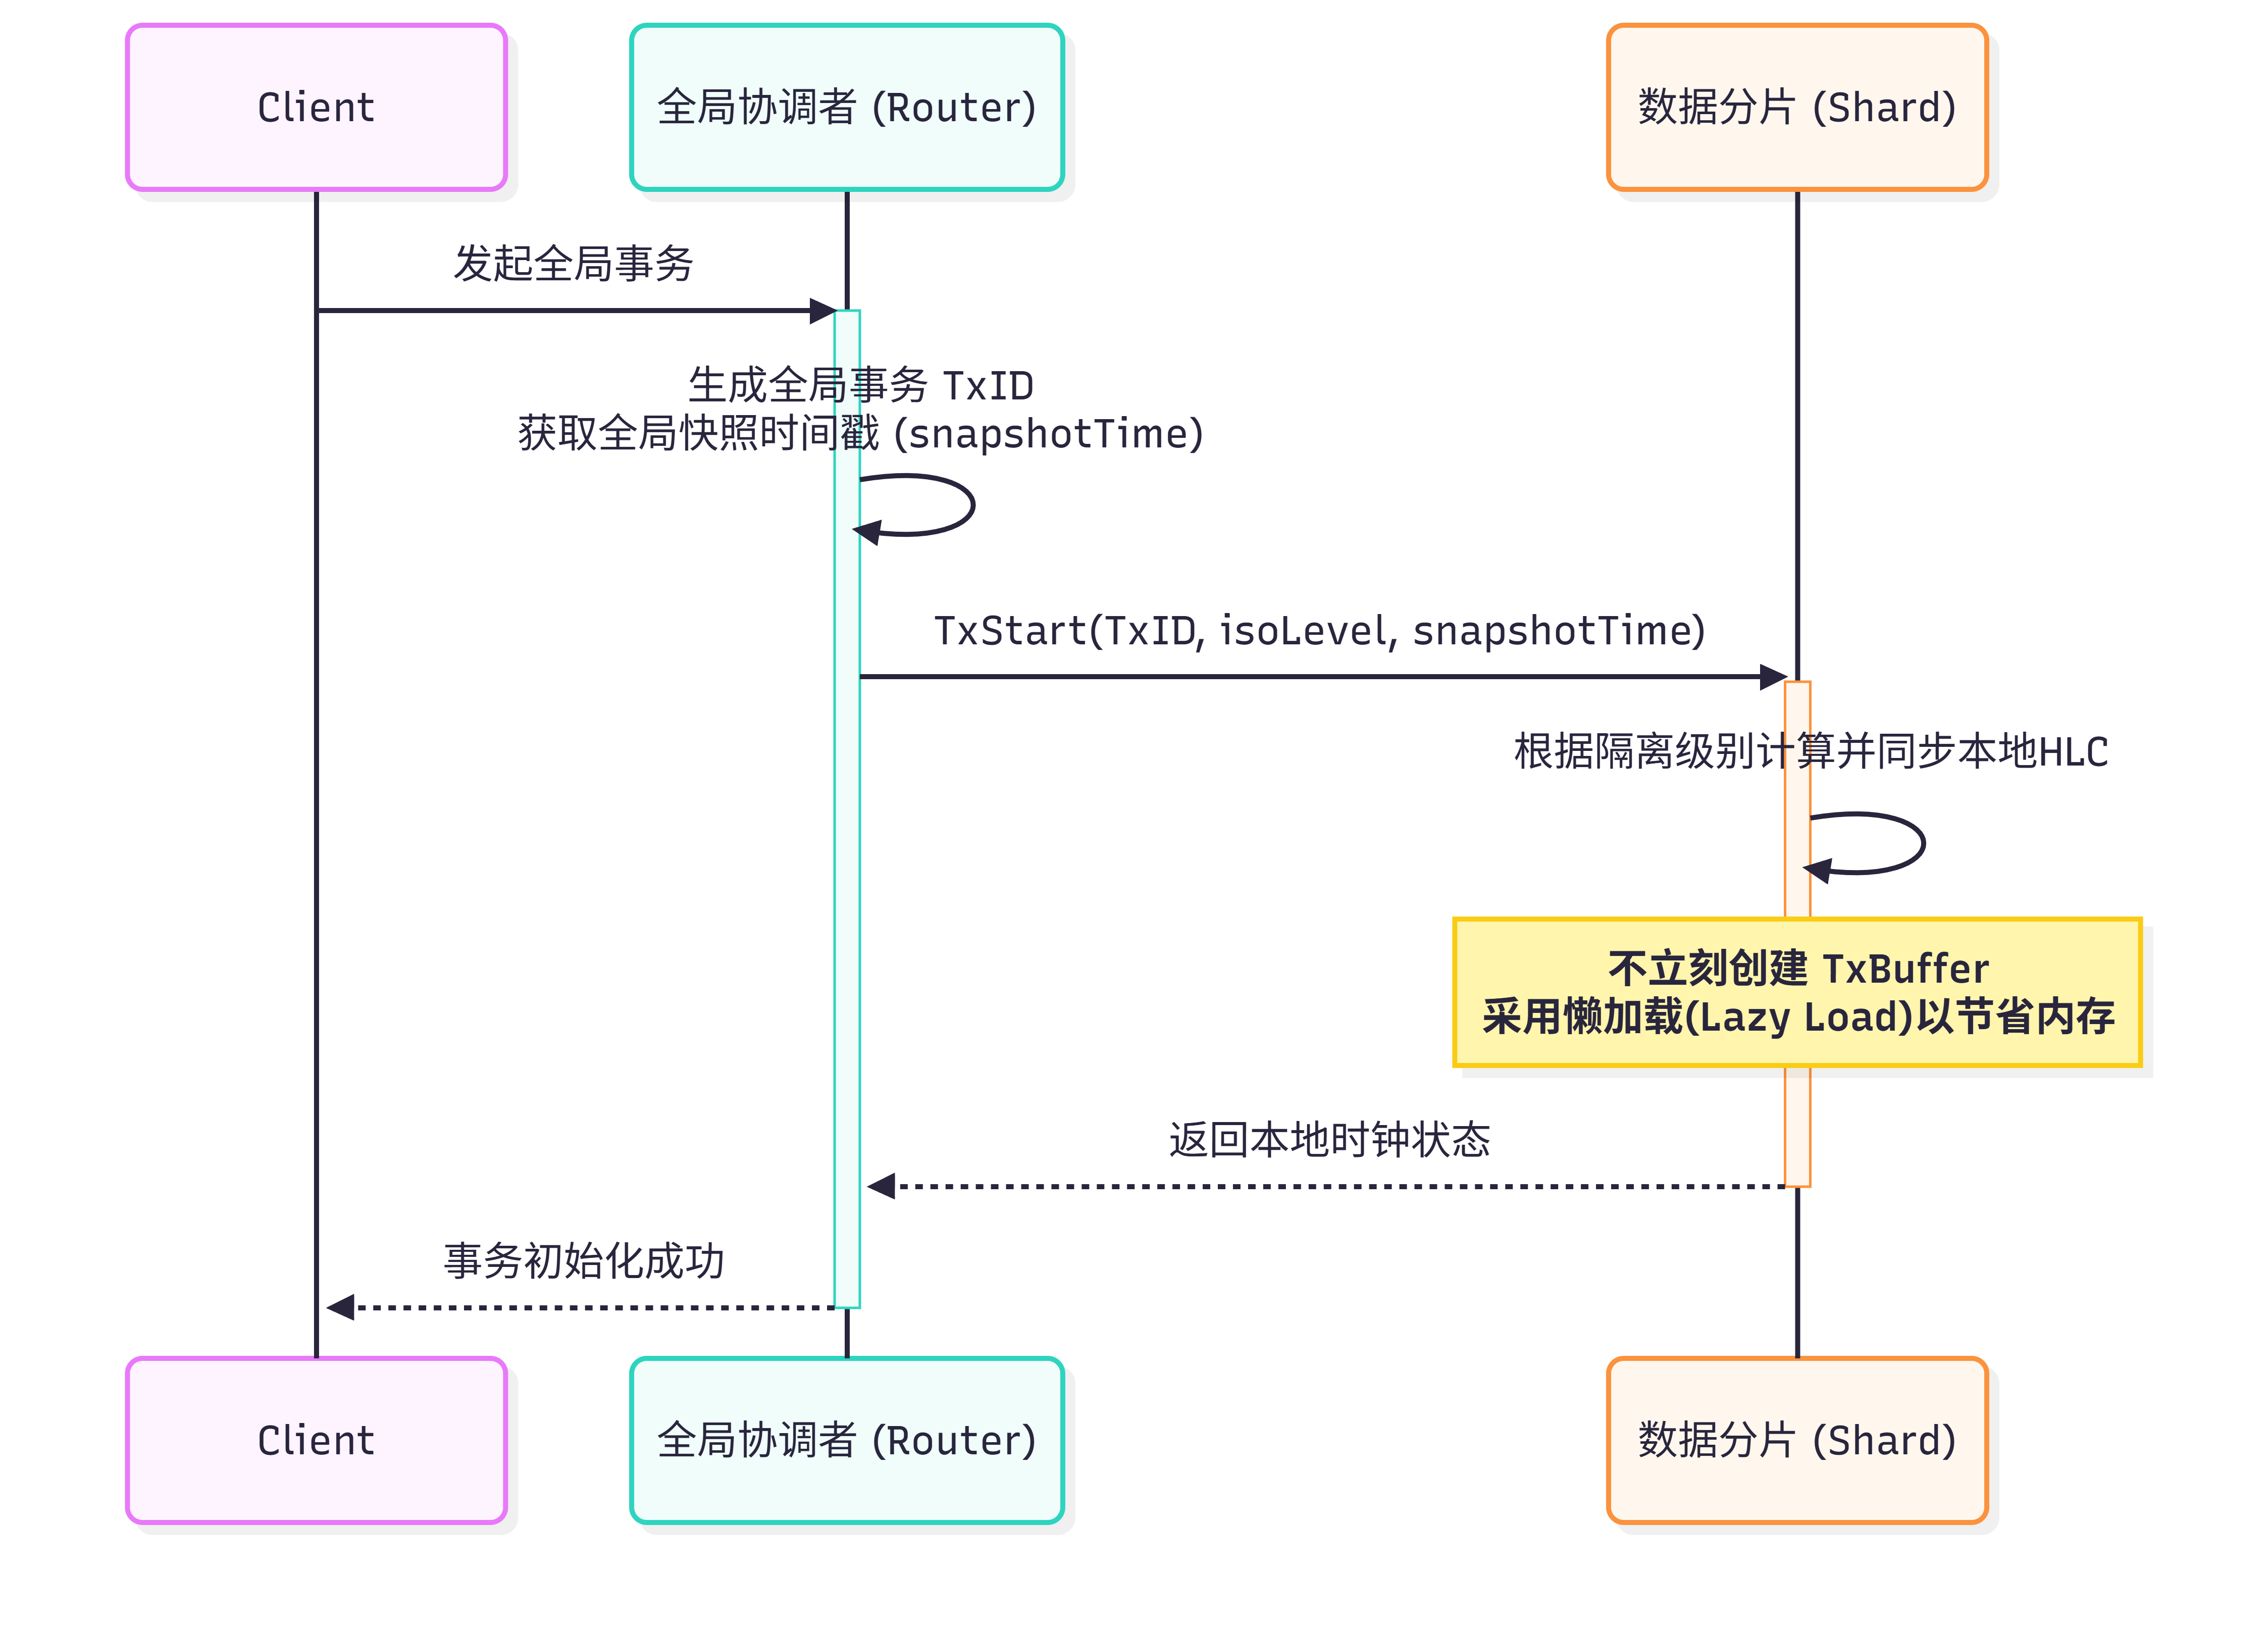
\includegraphics[width=0.8\textwidth]{figures/global-timeline.png}
    \caption{组件交互时序图}
    \label{fig:global-timeline}
\end{figure}

相对地，涉及具体分片的数据操作信息则通过分片内的 \lstinline|TxBufferManager| 进行局部维护。由于未决事务的读写集极可能导致极大的内存开销，代码在此处采用了懒加载（Lazy Load）机制：只有当该分片真正执行首次 \lstinline|TxRead| 或 \lstinline|TxWrite| 时，才会实例化对应事务的局部缓存（\lstinline|TxBuffer|）。这种分阶段存储策略大幅降低了分布式协同节点的通信负担，保证了内存状态的局部聚焦性。

\subsubsection{基于MVCC引擎的多版本读写流转}
分片底层的无锁化读并发依赖于多版本并发控制（MVCC）模型。以 \lstinline|TxRead| 为例，代码在读取数据时，严格遵循“读己之所写（Read-Your-Own-Writes）”的内部一致性：系统首先探测本地事务缓冲区的 Write 集合，命中后判断记录是否带有删除标记（Deleted）。如果本地无修改记录，读请求将穿透至底层的 \lstinline|MVCCStore| 操作对象，基于给定的 \lstinline|snapshotTime| 定位并获取小于但最接近该时钟的可用历史版本。

此外，程序还为最高隔离级别（SER）引入了悲观的锁机制转换。如果事务的隔离级别为 SER，分片内部将直接通过 \lstinline|lockMgr.AcquireRead| 强制索取分布式共享锁，在读写阶段即时屏蔽幻读和写倾斜缺陷，从而保证全局事务的严格串行化调度。

\subsubsection{两阶段提交可见性漏洞(Hole)的消除}
在标准的分布式两阶段提交（2PC）协议中，由于多个参与者节点的 \lstinline|Prepare| 阶段无法做到绝对原子同频，常存在所谓的可见性漏洞（Visibility Hole）——即事务虽然已经预定将要提交，但若并发的读取操作携带了更大（或相同）的时间戳进入，可能会因为读取到旧版本而破坏线性一致性。

\begin{figure}[htbp]
    \centering
    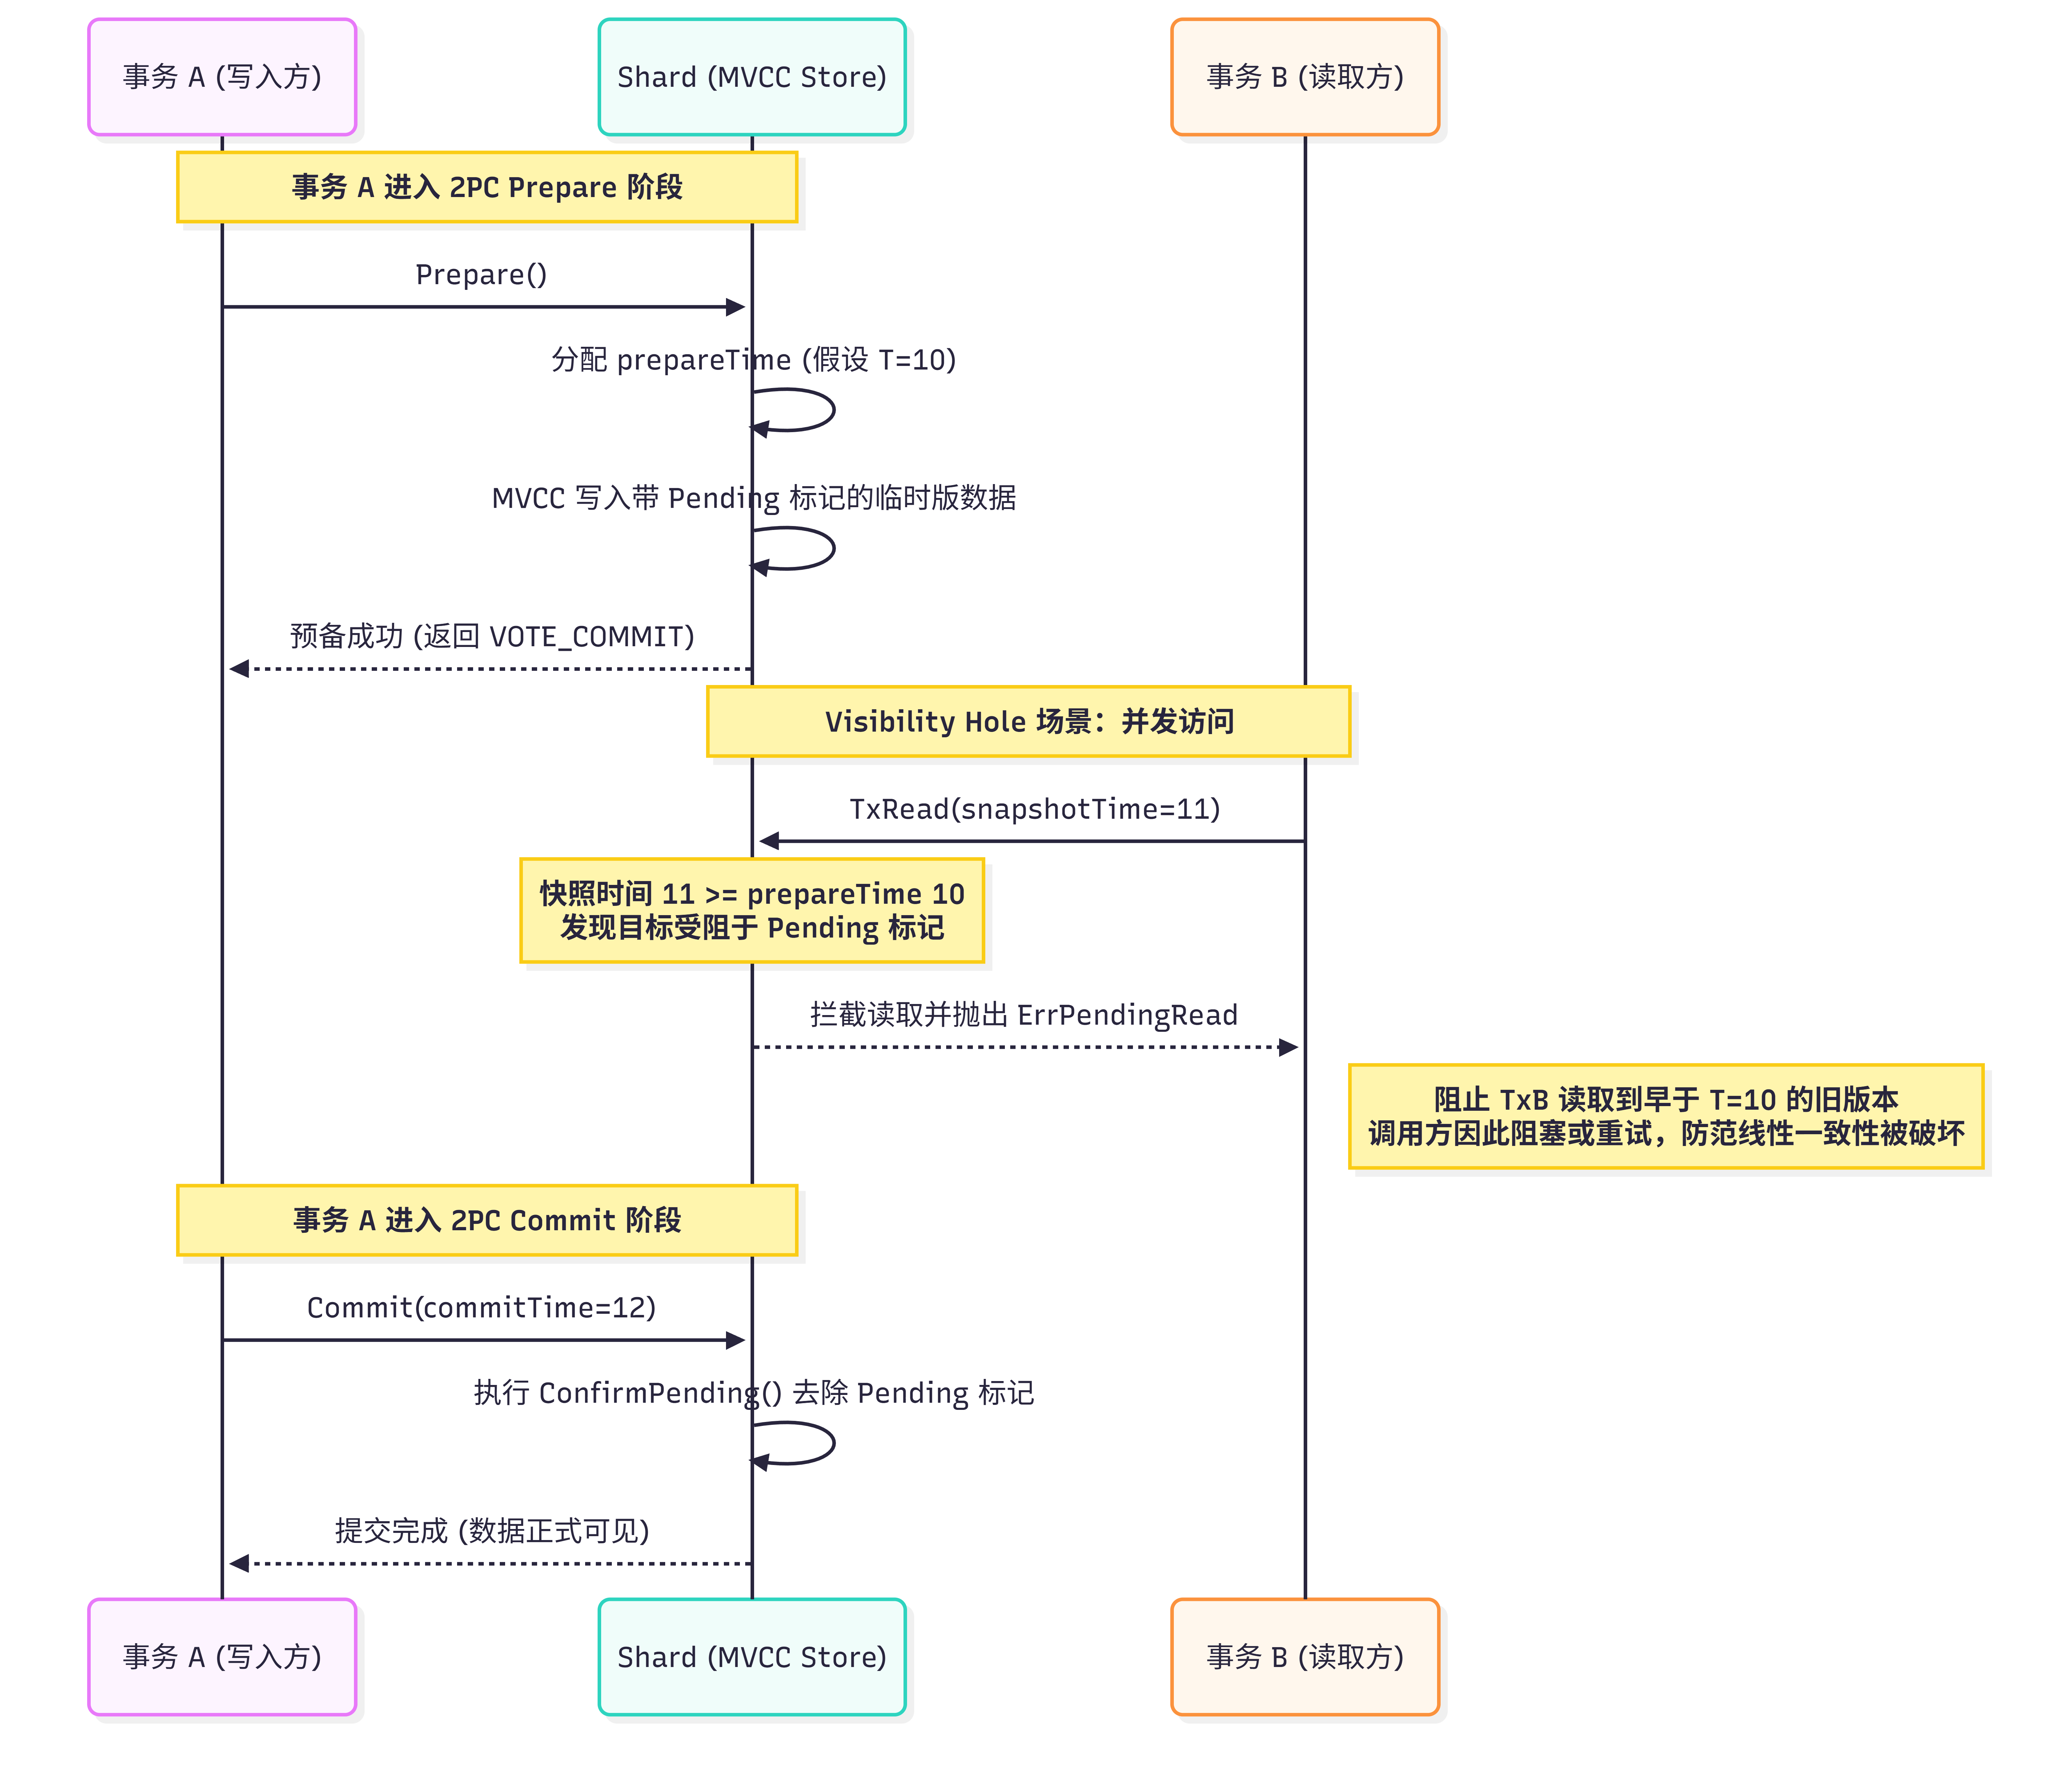
\includegraphics[width=0.8\textwidth]{figures/2pc-hole.png}
    \caption{两阶段提交可见性漏洞示意图}
    \label{fig:2pc-hole}
\end{figure}

本组件借助未决状态（Pending Status）与时间戳推进解决了该漏洞：系统在 \lstinline|Prepare| 阶段，根据混合逻辑时钟（HLC）派生出本地的预备时间 \lstinline|prepareTime|。此时并未直接覆盖老数据，而是调用 \lstinline|store.Put| 打上 Pending 标记以及临时版本号。这一预写行为充当了并发读操作的前向屏障：倘若并发读查询的时间戳满足 $\lstinline|snapshotTime| \ge \lstinline|prepareTime|$ 并且遇到了 Pending 标位，底层将抛出 \lstinline|ErrPendingRead|。这一拦截行为促使过早发起读取操作的调用方陷入阻塞或执行安全重试。直至最终协调者下达任务并在 \lstinline|Commit| 函数内通过 \lstinline|store.ConfirmPending(txId, commitTime)| 将版本信息实化确立，系统的时钟推进即可闭环，可见性漏洞得以彻底消除。

\subsubsection{事务降级与单分片快速提交(QuickCommit)优化}
当系统规划器判定当前事务的作用域仅局限于某单一分片时，该组件会触发 \lstinline|QuickCommit| 的快速提交路径，以规避2PC的网络协商与多次RPC的延迟开销。
\begin{figure}[htbp]
    \centering
    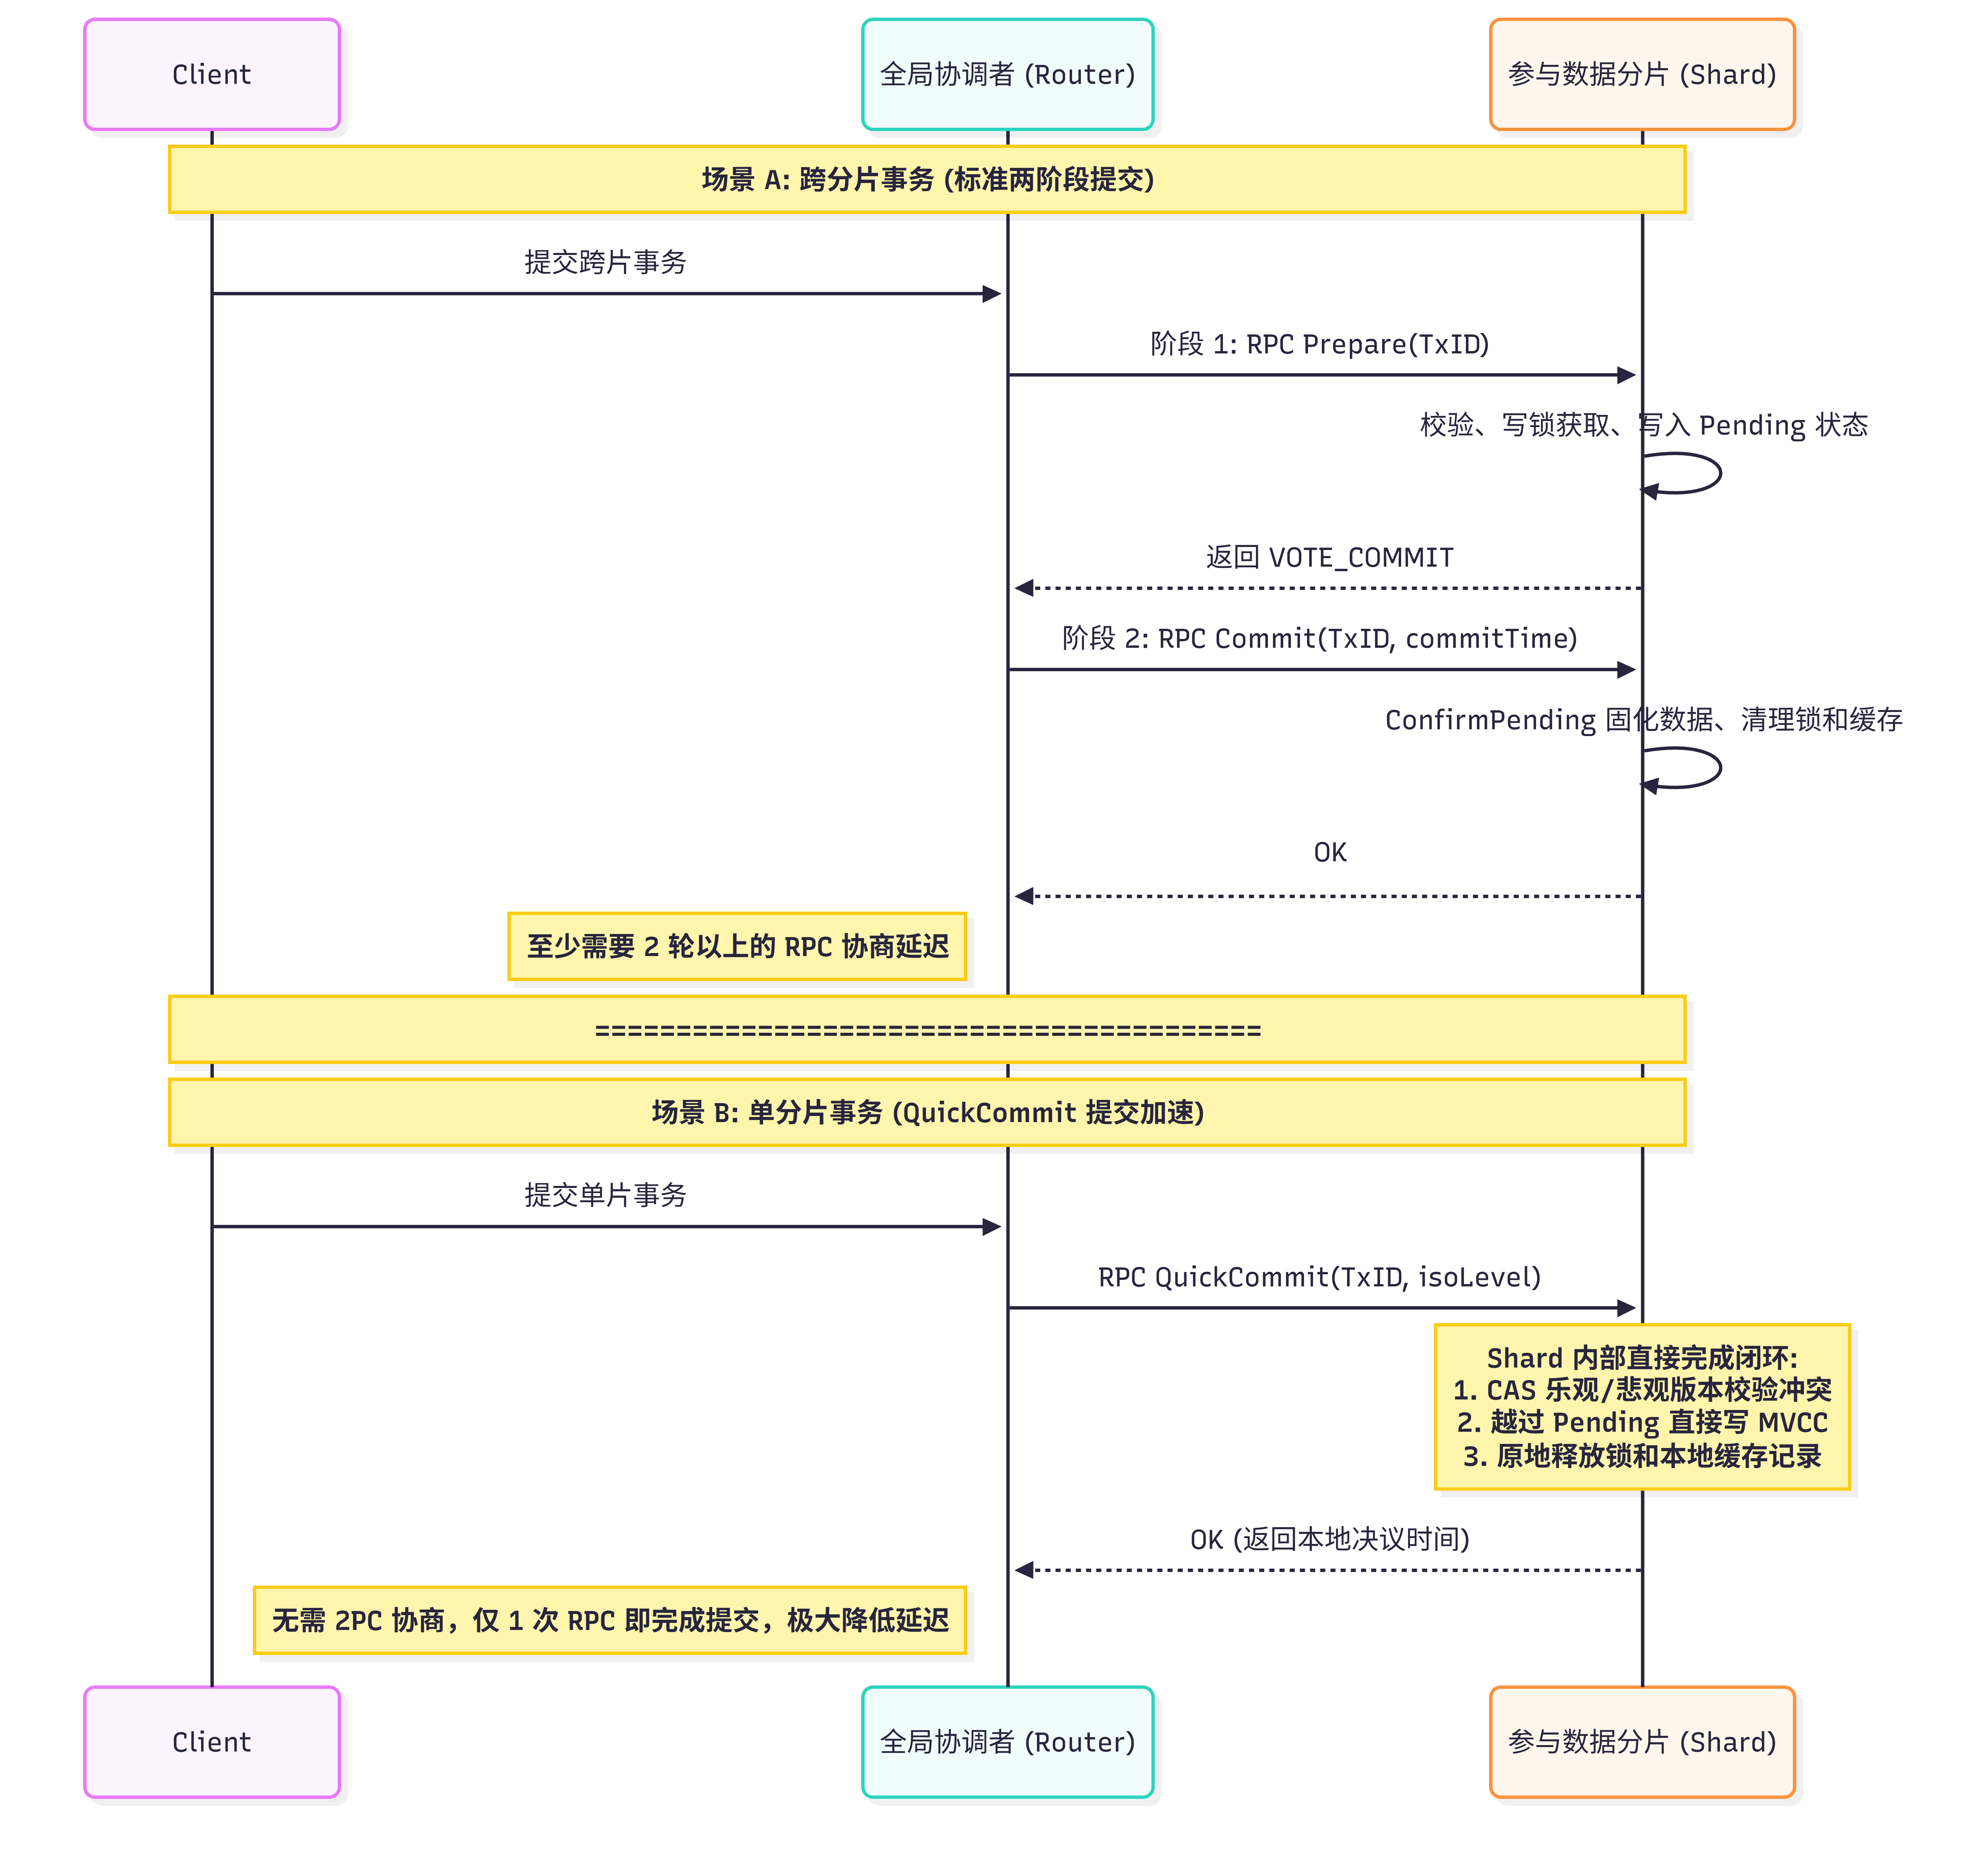
\includegraphics[width=0.8\textwidth]{figures/quick-commit.png}
    \caption{组件交互时序图}
    \label{fig:global-timeline}
\end{figure}

在 \lstinline|QuickCommit| 的实现逻辑中，由于剔除了 \lstinline|Prepare| 阶段，事务的操作直接收敛为单次原子变更：引擎首先基于 \lstinline|clock.Tick()| 获取即时的决议时间；随后的 CAS 校验模块针对 PSI/SI 以及 SER 隔离级别执行乐观并发验证，确保持有缓冲区数据的 \lstinline|OriginalVersion| 仍然是当前系统中的最新版本以防覆盖写入。在通过版本校验且获取必要的本地写锁之后，\lstinline|QuickCommit| 将直接跳过 Pending 预写入流程，把缓冲池内的数据带有完整的 \lstinline|commitTime| 非挂起标志（将 pending 设为 \lstinline|false|，原版本置为 \lstinline|0|）径直向 MVCC 底层固化。由于校验、写入、提交与释放锁在单一分片层级形成了一个闭环，在保障 ACID 语义不被破坏的前提下，极大提升了单分片事务的并发吞吐能力。

\subsection{路由节点事务状态机实现}

\subsection{系统容错与可观测性}

\section{本章小结}